% !TEX root = ../main.tex

\section{Result}
function if you look at the phase shift you can see a difference in phase shift from the different frequencies,
this is just honorable in the output of the delay function.


\begin{figure}[!hbt]
	\centering
	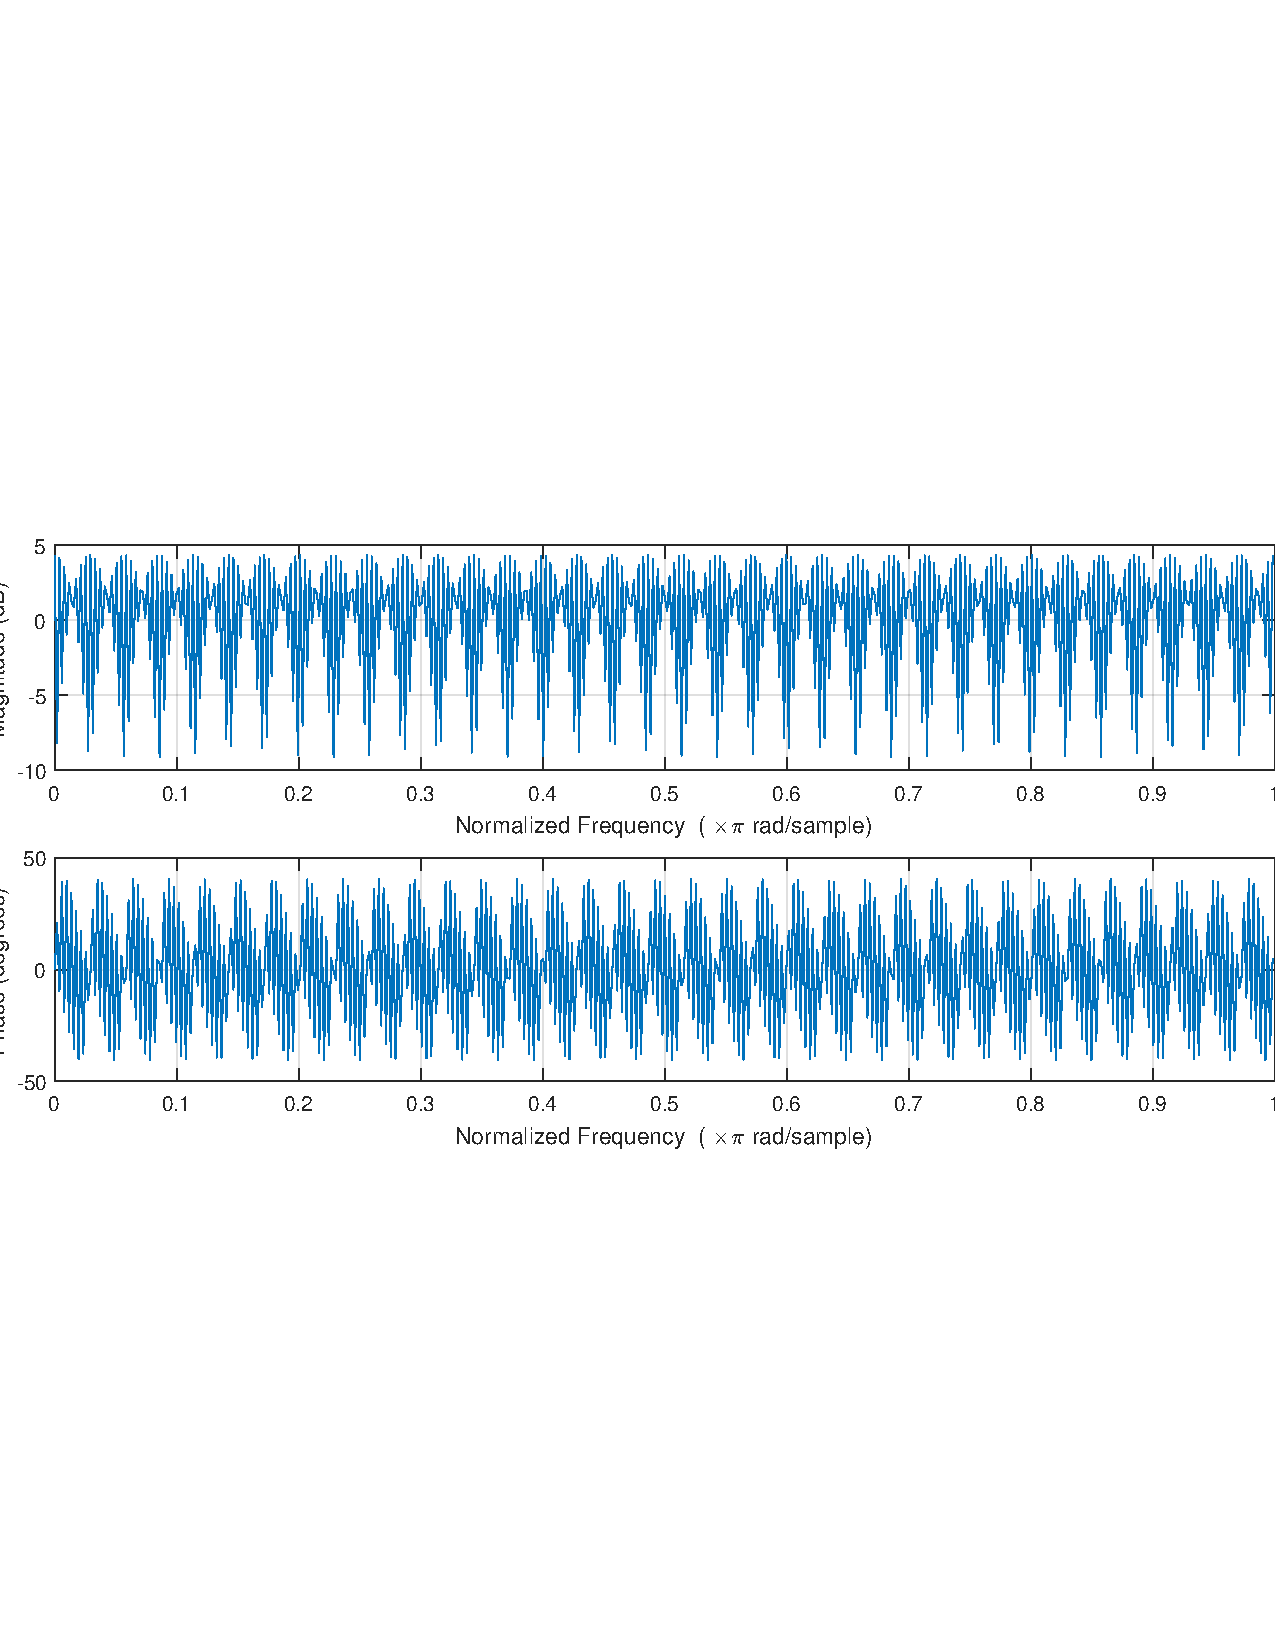
\includegraphics[width=\textwidth]{filter_characteristics.pdf}
	\caption{shows the response of the delay filter.}
	\label{fig:response}
\end{figure}


In the chorus effect, when you compare the 2 sound clips the one before the courts affect is added and the one after.
You notice a more smoothness of tone and the sound of extra trumpets especially jumps out at you which really gives the appearance of grandeur.
